\documentclass[10pt]{article}
 
\usepackage[margin=1in]{geometry} 
\usepackage{amsmath,amsthm,amssymb, graphicx, multicol, array}
\usepackage{enumitem}
\usepackage{hyperref}
 
\newcommand{\N}{\mathbb{N}}
\newcommand{\Z}{\mathbb{Z}}
 
\newenvironment{problem}[2][Problem]{\begin{trivlist}
\item[\hskip \labelsep {\bfseries #1}\hskip \labelsep {\bfseries #2.}]}{\end{trivlist}}

\date{Due: Sep 13, 2022 10pm PT}

\begin{document}
 
\title{Assignment 2}
\author{
CS 181AG: Network Algorithmics}
\maketitle

This assignment will help you understand how to extend LANs. It includes a coding component, short-answer questions related to your code, and a reading assignment with questions.  

 
\begin{problem}{1: Learning Bridges}
Assignment2.py simulates creating 5 LANs, with a total of 7 nodes attached to them and 2 bridges, each containing three ports,  connecting them. It will be very helpful to you to draw the setup.

\begin{enumerate}
    \item After you've taken some time to familiarize yourself with the code, send a message from A to B by adding to the bottom of main: ``A.send\_message(B)''. List all the nodes that hear the message, whether it was intended for them or not (you need not include the sender). Then, send a message from B to A. List all the nodes that receive the message, whether it was intended for them or not. Why is this inefficient? What is the key functionality of bridges that is missing?
    \item Fix the above issue by editing the ``receive\_message'' function in the Bridge class. You may add any necessary variables to the class. Now repeat the two steps from \#1 and for each, list the nodes that hear the message. This is the final version of your code.
    \item Draw the state of B1 and B2's learning tables after both these messages are sent. 
    \item For each of the following, list the nodes that hear the message and draw the learning tables for B1 and B2. If your implementation is correct, you \emph{can} simply add print statements and run your code to get these answers. However, for practice, I encourage you to solve them using your own logic and then verify using your code. 
    \begin{enumerate}
        \item E sends a message to A
        \item C sends a message to F
        \item D sends a message to F
        \item B sends a message to C
    \end{enumerate}
    
    \item For the next sub-question, \textbf{assume all learning tables are empty and we have not run the spanning tree protocol}. Describe briefly what would happen if we added another bridge, B3, and another LAN L6, with B3's port-to-LAN mapping {P1: L2, P2: L3, P3: L6}, and then sent a message from C to D.
\end{enumerate}
\end{problem}
\begin{problem} {2: Spanning Tree}
\begin{enumerate}
    \item Consider the practice problem from class (slide 34). We decided that when running the spanning tree protocol, B3, B6, and B7 had one of the ports shut off. For B3, write out the messages it would send and receive (and to/from which bridges) until convergence (i.e., messages don't change), following the format from class (Me, Root, Hops). To start: 
    
    Round 1:
    
    Send: (B3, B3, 0) to B2 and B5
    
    Receive: (B2, B2, 0) from B2
    
    Receive: (B5, B5, 0) from B5
    
    Round 2:
    
    ...
    
    
   \item Repeat the above for bridge B7.
   \item The Spanning Tree Protocol was invented by Radia Perlman, one of the internet pioneers who also loved writing and composing music. \href{https://www.youtube.com/watch?v=iE_AbM8ZykI}{Here} she is, sharing the STP with the world. No work here, just for your enjoyment :)
    
\end{enumerate}
\end{problem}
\begin{problem}{3: Reading}
The pandemic has sparked a recent debate about whether the internet should be treated and regulated like a public utility. A quick Google search should give you plenty of articles supporting each side. Read one article in support of treating the internet like a public utility and one against. Paste both urls and summarize the main points for each. Write a couple sentences articulating your thoughts after reading both. Points are for effort.
\end{problem}
\begin{problem}{4}
How long did this assignment take you?
\end{problem}
\begin{problem}{5: Extra (optional) reading}
\href{https://www.pewresearch.org/internet/2021/09/01/the-internet-and-the-pandemic/}{Here} is a Pew Research Center article about how Internet usage (both numbers and sentiments) changed during the pandemic. It also includes some stats about equity in internet access. There is no work or credit or extra credit associated with reading this - just more information if it interests you. 
\end{problem}

\newpage

\subsection*{Answers}
    \begin{enumerate}
       \item \begin{enumerate}
        \item If we are sending a message from $A$ to $B$, the following nodes hear the message: B, C, D, E, F, G. This is the same situation for if we send from $B$ to $A$ (B, C, D, E, F, G all see the message). This is inefficient since B recieved the message meant for them first, but the message remained on the line and all other nodes heard the message, thus meaning that a message was on the line for far longer than necessary. The key functionality of bridges that is missing is selective forwarding which would prevent the "flooding" of messages to the other LANs.
        \item Fixing the issue, the node that recieves the message from $A$ is $B, C, D, E, F, G$, and the only node that receives the $B$'s message is $A$. This is efficient, since the bridge learns which port $A$ is at from the prior message and can selectively forward (this time not forwarding) accordingly. There is no need for any of the other nodes to hear the correspondance between the two of them.
        \item 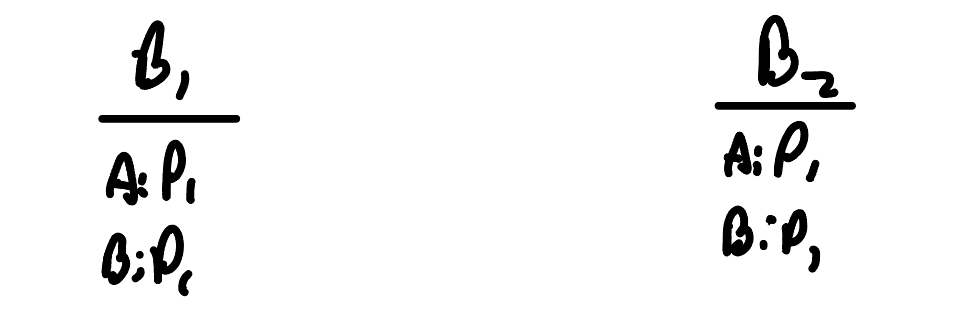
\includegraphics[scale = 0.2]{hw2p13.jpeg}
        \item 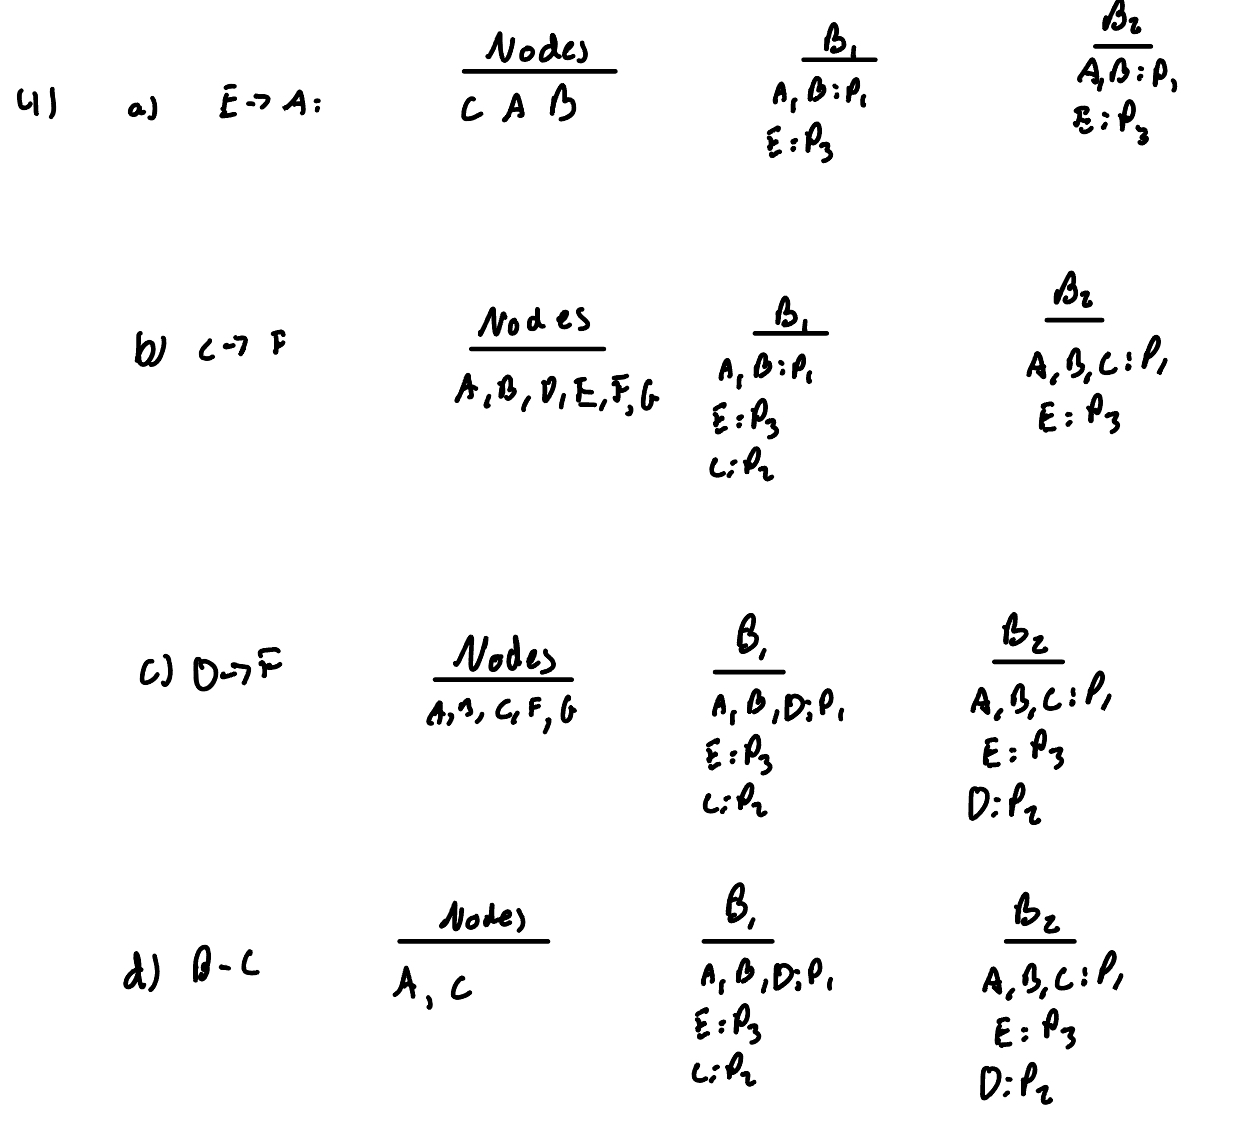
\includegraphics[scale = 0.2]{hw2pr14.jpeg}
        \item With the insertion of the new bridge and new LAN, we can see from the graph topology that we no longer have a tree as we now have a cycle that goes B1-$>$L1-$>$B2-$>$L3-$>$B3-$>$B1. Therefore, since all learning tables are empty and we have not run our spanning tree protocol, we can note that we would have an infinite loop of sending messages along the lines.
       \end{enumerate}
       \item \begin{enumerate}
        \item Round 2:\\
            Send: (B3, B2, 1) to B5\\
            Receive: (B2, B1, 1) from B2\\
            Receieve: (B1. B5, 1) from B5\\
            Round 3 (Final and does not change):\\
            Status: (B3, B1, 2)
            Receive: (B2, B1, 1) from B2\\
            Receive: (B5, B1, 1) from B2
        \item Round 1:\\
            Send: (B7, B7, 0) to B5, B1\\
            Receive: (B1, B1, 0) from B1\\
            Receive: (B5, B5, 0) from B5\\
            Round 2:\\
            Send: (B7, B1, 1) to B5\\
            Receive: (B1, B1, 0) from B1\\
            Receive: (B5, B1, 1) from B5\\
            Final State:
            Status: (B7, B1, 1)
       \end{enumerate}
       \item\begin{enumerate}
       \item \href{https://www.forbes.com/sites/forbestechcouncil/2020/06/17/the-argument-for-the-internet-as-a-utility-is-it-time-to-change-how-its-delivered/?sh=4a8c34467729}{Pro-treating the internet as a utility}: The COVID-19 pandemic displayed the inequalities that would stem from inaccessability to the internet, such as discrepencies in the access to information, services, and cultural phenomenas that have come as a result of the digitization of our lives. Similarly, the current capitalistic model of internet access has short-comings in the sense that it is not profitable for internet companies to provide massive broadband support which hampers access. However, in order to fully allow the internet to become a commodity, it is important that we invest in proper infrastructure so that way all communities can reap the benefits of the utility, as the purpose of making the internet be a public utility is to make internet access more equitable. I think that this article makes a number of good points in the sense that there is a clear issue with the equitability of access to the internet that was especially exemplefied during the COVID-19 pandemic. However, to immediately argue for the need to make the internet a public utility seems to me to be a drastic step, as it would make more sense to me to provide subsidies to provide internet access in particular areas and to upgrade existing systems. As of right now, there does not seem to be price gouging in the markets for internet access (at least that I have seen/experienced) which in my opinion, would more clearly warrant these types of actions. The internet is something that definitely should be available for all to consume and utilize for their safety and entertainment but I do not agree with the argument that the answer is to make it a public utility.
       \item \href{https://www.washingtonpost.com/news/innovations/wp/2016/07/07/why-treating-the-internet-as-a-public-utility-is-bad-for-consumers/}{Anti-treating the internet as a utility}: The perscription of a "public utility" upon a particular service, as has been demonstrated to be the FCC's intentions with the internet eventually. However, this is not done with the intention of providing the best experience for the consumer and is a misguided use of regulation and monopolistic preventitive measures in a situation that is not warented. The internet can be provided to consumers by numerous different providers and lower costs and higher speeds than a majority of countries that have made the internet a public utility. This decision would also result in anti-capitalist measures such as a ceasing of innovation that would also be adding onto a poor American infrastructure that has shown an inability to be maintianed to a high standard that would be available via private enterprises. In essence, the article argues that the issue with making the internet a public utility is the ceasing of capitalist factors that spur innovation. Akin to the other article in favor, I agree with a number of the points made by the auther, specifically with the idea that the natural competition in the industry over internet access seems to be working the way that capitalism intends and that American public utilities have displayed many weakenesses with respect to complacencies such as we have seen with the energy industry in Texas. However, this article seemed to me to take a laisez-faire approach to answering the question which I do not agree wholeheartedly with. I personally believe that there can be innovation and the market competitiveness that have driven internet development while taking governemntal and regulatory measures to ensure that access to internet is more equitable and helping private companies improve their existing grids through government intervention.
       \end{enumerate}
       \item This homework took me $\approx 8$ hours
        \end{enumerate}
\end{document}